%!TEX root=../master_thesis.tex

\chapter{Riak Core Lite and Random Slicing}
This chapter covers how the architecture and behavior of \ac{RCL} was changed while replacing Consistent Hashing with \ac{RS}.
First we give an explicit recapture of the responsibilities and guarantees of Consistent Hashing in \ac{RCL}, how \ac{RS} compares in those aspects, and what open problems directly follow from this comparison.
Analogous to Section \ref{sec:riak_core_lite} the next sections contain changed and new components as well as system actions that changed.

\section{Comparing Consistent Hashing and Random Slicing}
In \ac{RCL} Consistent Hashing provides a homogeneous partitioning of the ring.
Together with the claim algorithm it guarantees that for each partition the $N$ successor partitions are owned by $N$ distinct nodes if there are enough nodes in the cluster.
This enables a simple and fast computation of the preference list.
The indices on the ring are fixed unless a special resize operation is executed.
We visualize the difference between the ring structures in Figure \ref{fig:chash_and_rslicing}.

On the other hand \ac{RS} partitions the ring into dynamic sections.
It does not give a guarantee on the order of owners and therefore does not enable a simple and fast computation of the preference list.
Since the partitioning of the ring happens dynamically there is no resize operation.

From this one can conclude that open problems are the computation of the preference list and if there are changes that originally happened during the resize operation and are still relevant and therefore need to be applied elsewhere.
We discuss solutions for the computation of the preference list in Section \ref{sec:replication_placement_strategy} and other open problems are discussed in the appropriate places in the following sections.

\begin{figure}
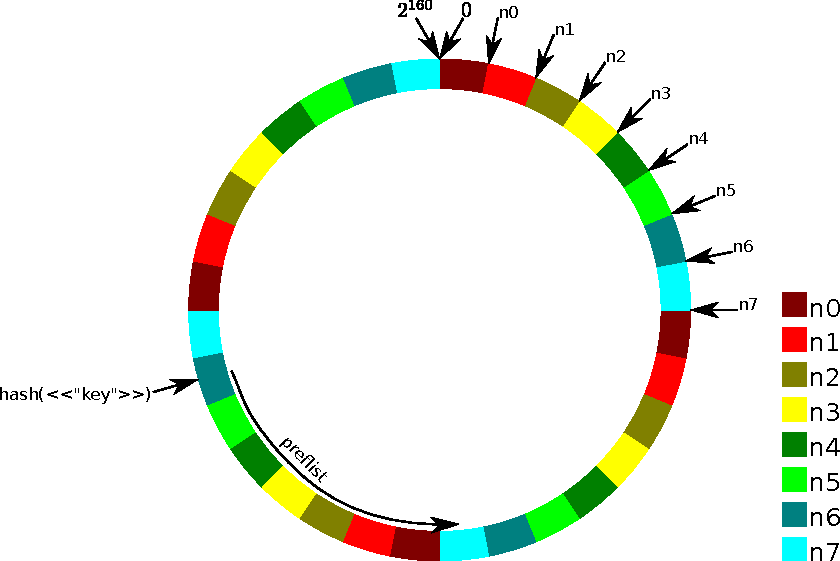
\includegraphics[width=0.5\textwidth]{consistent_hashing_example}
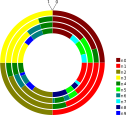
\includegraphics[width=0.5\textwidth]{random_slicing_example}
\caption[Side by Side Comparison of Consistent Hashing and Random Slicing]{Side by Side Comparison of Consistent Hashing and Random Slicing. On the left one can see the homogeneously partitioned Consistent Hashing ring while on the left one can see the dynamic changes in the \ac{RS} ring.}
\label{fig:chash_and_rslicing}.
\end{figure}


\section{Changed Components}
In this section we explain how the components listed in Section \ref{sec:replication_placement_strategy} were changed during the integration of \ac{RS} both with respect to their responsibilities as well as their basic functionality.
Any component that is not mentioned in this section was left unchanged or only changed on a technical level.

\subsection{Ring}
On an abstract level there are only minor changes in the ring component.
The model of the ring changed to that of \ac{RS} and therefore the computation of the preference list is now solely relying on the navigation component.
As the indices are not fixed in the new ring model the ring reconciliation algorithm had to be overhauled and relies now on choosing the most up-to-date ring and adding all missing members to it via the \ac{RS} algorithm.

\subsection{Navigation}
\label{sec:navigation_rslicing}
The navigation component had to be reworked almost completely.
First of all, the Consistent Hashing model at its core was replaced by an adaptation of Scott Fritchie's \ac{RS} implementation (see Sec \ref{sec:partitioning_algorithm}).
From that it directly follows, that the preference list cannot be computed by iterating over the successor nodes in the ring.
Instead the component uses the \acp{RPS} we present in Section \ref{sec:replication_placement_strategy}.
This also leads to strong restrictions on the use of the optimized read-only structure this component uses as it cannot be used to compute the preference list.

\subsection{Claim}
As the core component of the claim component the claim algorithm is obsolete as load balancing on the ring is directly achieved by Random Slicing.
Since the claim component is also responsible for the stage-plan-commit life cycle it still stays relevant and is the entry point for changes to the ring.
Instead of applying the claim algorithm in the commit phase the new ring is computed by using \ac{RS} with the old ring and new cluster configuration.
Through this it is assured the new guarantees given by the \ac{RS} model are fulfilled in the actual ring.


\section{Changed System Procedures}
In this chapter we explain the changes we made to the system procedures while integrating \ac{RS} with Riak Core.
Procedures that are mentioned in Section \ref{sec:system_procedures} but do not appear in this section are not changed significantly.

The system still uses the stage-plan-commit life-cycle for cluster changes. The stage phase has not changed as the cluster changes are still marked in the ring and gossiped to all members.
However, in the commit phase the updated ring is now computed by simply applying \ac{RS} to the old ring with the new member configuration.

\subsection{Leave Cluster}
The procedure of leaving the cluster remains unchanged in the most parts.
However, the leaving node is now actually removed from the ring on the next update-ring-event instead of the next claim execution.

\subsection{Navigate the Ring}
As we mentioned in Section \ref{sec:navigation_rslicing} the navigation component only offers reduced functionality with the optimized binary structure.
The removed functionalities include computing the preference list via that structure.
It now uses the ring model directly.
This does not restrict the functionalities of the navigation component but it may have a negative impact on the performance.
Other procedures navigating the ring were only changed in the aspect that they now use the \ac{RS} ring model together with the new replication placement algorithms.

\subsection{Resize Ring}
As there is no fixed ring size and the ring structure is changed with every cluster change there is no explicit resize operation anymore.
In the current state of the system any optimization and corner case handling in the handoff and ring update procedures during a resize operation is lost.

\subsection{Handoff}
While the actual execution of the handoff from the old owner of an index to the new owner has not changed the preparation of the handoff has changed significantly.
As the ring has no fixed indices anymore it has to be assured that there are virtual nodes running for all old and new indices.
This is achieved by computing a handoff-ring from the old and new ring that includes all indices of both rings and each index is owned by the onwer that would own it in the old ring.
This procedure is visualized with an example in Figure \ref{fig:handoff_ring}.
From this handoff ring the correct virtual nodes are running and can start the handoff procedure as usual.
When there are two neighboring sections owned by the same physical node the sections are merged on the next ring-update-event.

\begin{figure}
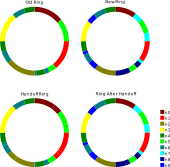
\includegraphics[width=\textwidth]{handoff_ring}
\caption[Handoff Ring]{Handoff Ring. First the indices of the old and new rings are merged and then assigned to the old owners. After the handoff the new ring results.}
\label{fig:handoff_ring}
\end{figure}